
%Introduce the NOvA detectors and give big picture overview
The NOvA experiment (NuMI Off-axis $\nu_e$ Appearance) consists of two
detectors which measure the neutrino composition of the NuMI
(Neutrinos at the Main Injector) beam. The
300~ton near detector is located on site at Fermilab 1.015~km 
from the NuMI
target. The 14~kiloton far detector is located at a site near Ash
River Minnesota and is 810km from the
NuMI target. Both detectors are placed off-axis from the centre
of the NuMI beam by 14.6~mrads.

The original design of the NOvA experiment is laid out in the
technical design report (TDR) \cite{TDR}. The constructed experiment
differs only slightly with the design laid out in the TDR. The details
of the constructed experiment, including the neutrino beam source and
the two detectors, are discussed in the following chapter.


\section{The NuMI Beam}

The NOvA experiment's neutrino source is provided by the Neutrinos at
the Main Injector (NuMI) beam at Fermilab. The following section
describes the process by which the NuMI muon neutrino beam is created.

An instructive diagram of the NuMI beam facility is presented in
Figure~\ref{fig:NuMI}.
The Main Injector accepts six batches, each spanning 10~$\mu$sec, of
protons at a time and accelerates the protons up to 120~GeV. A 10~$\mu
s$ pulse of accelerated protons, known as a beam spill, is directed to
collide with the 95~cm long graphite target every 1.33~s. 

The collision of the accelerated protons with the carbon atoms of the
target produce a plethora of secondary particles (mostly pions and
kaons). The charged
mesons are focused into a beam by two magnetic focussing horns. 
The focussed beam of charged mesons then travels through a 675~m long
evacuated decay pipe. Along this length of pipe the mesons decay
predominantly to charged leptons and neutrinos. 
The decay pipe is followed by hadron and muon
monitors and about 240m of rock. The rock absorbs the remaining charged
particles in the beam before reaching the near detector.

Details of the focussing horns and off-axis detector detector position
are provided in the following subsections.

% NuMI beam figure
%\begin{figure}[!ht]
\begin{figure}
  \centering
  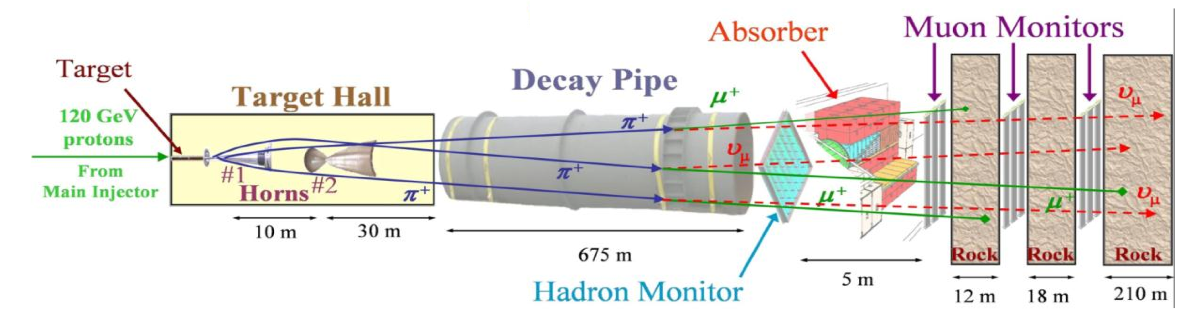
\includegraphics[width=1\textwidth]{../../img/beam/beam_diagram.png}
  \caption{A diagram showing the layout of the NuMI beam.}
  \label{fig:NuMI}
\end{figure}

\subsection{Focussing Horns}

Focussing horns are used to focus the mesons, created by collisions of
protons with the NuMI target, into a beam. Changing the current
direction within the magnetic focussing horns changes the sign
of the mesons that are focussed. The focussing horns are run in
Forward Horn Current (FHC) or Reverse Horn Current (RHC)
mode to select positively or negatively charged mesons
respectively, leading to a neutrino or an anti-neutrino beam respectively. 


\subsection{Off-axis Detectors}

The NOvA detectors are both placed 14~mrads off the axis of the NuMI
beam.
The reasons for placing the detector will be described
in more detail in the following paragraphs. 

The decay used to produce a neutrino beam is a two body decay, where a
pion (or kaon) decays to a neutrino and a muon. The two body decay 
occurs isotropically in the parent particles rest frame. 
In the lab frame the parent particle is not at rest when decaying. For
pion and kaon decay this boosts the neutrinos into a cone in the
direction of the parent particle.
For small angles, the flux and energy of neutrinos produced by pion
decay ($\pi \rightarrow \nu_{\mu} + \mu$) are given by:

\begin{equation}
\Phi = \left( \dfrac{2\gamma}{1+\gamma^2 \theta^2} \right)^2 \dfrac{A}{4\pi z^2}
\label{eqn:NuPiFlux}
\end{equation}

\begin{equation}
E_{\nu} = \dfrac{0.43E_{\pi}}{1+\gamma^2\theta^2},
\label{eqn:NuPiEnrgy}
\end{equation}

where $E_{\pi}$ is the energy of the parent pion, $m_{\pi}$ the mass of the
parent pion, $\theta$ the angle between the pion and neutrino
directions and $\gamma = E_{\pi}/m_{\pi}$.

Equations~\ref{eqn:NuPiFlux}~and~\ref{eqn:NuPiEnrgy} and are shown as 
functions of neutrino energy and off-axis angle in
Figure~\ref{fig:NuPiFlux}.
Figure~\ref{fig:NuESpectra_MEAndLE} shows the number of neutrino
events as a function of the
charged current $\nu_{\mu}$ energy for the Low (left plot) and
Medium (right plot) Energy Tune for various off-axis angles. 

For the Medium Energy Tune, figure~\ref{fig:NuPiFluxb} shows that at
14~mrad the neutrino energy
does not have a strong dependence on the parent pion energy.
In addition, figure~\ref{fig:NuESpectra_MEAndLE_b} shows that at
14~mrad the Medium
Energy Tune produces a narrow energy neutrino beam with approximately
4 times more neutrinos at 2GeV than the on-axis scenario. This peak at
2~GeV is well matched to the expected energy of the oscillation
maximum. The oscillation maximum for electron neutrino appearance in a
muon neutrino beam is expected to occur at 1.6~GeV for
NOvA's L/E and for $\Delta \textrm{m}_{32}^2=2.4~\textrm{meV}^2$.

As described above, placing the detector off-axis increases the flux
at the expected oscillation maximum. In addition the narrow energy
range of the off-axis beam improves the rejection of background
events. Neutral current events are an important background source
whose topologies can be hard to distinguish from electron showers
produced by $\nu_e$ CC events. For NC events the neutrino carries a
significant amount of the energy away and the visible energy tends to
''feed down'' to lower energies. For narrow band off-axis  beam this
feed down tends to shift the neutral current events to lower energies
outside the $\nu_e$ appearance signal energy window. Figure~\ref{fig:NuMIBeamComp}
shows the number of $\nu_{\mu}$, $\nu_e$ and NC events as a function
of visible energy, the bulk of the NC events (black histogram) are shown to shift below
the signal region (red-hatched histogram).


\begin{figure}
  \centering
  \begin{subfigure}[b]{0.45\textwidth}
  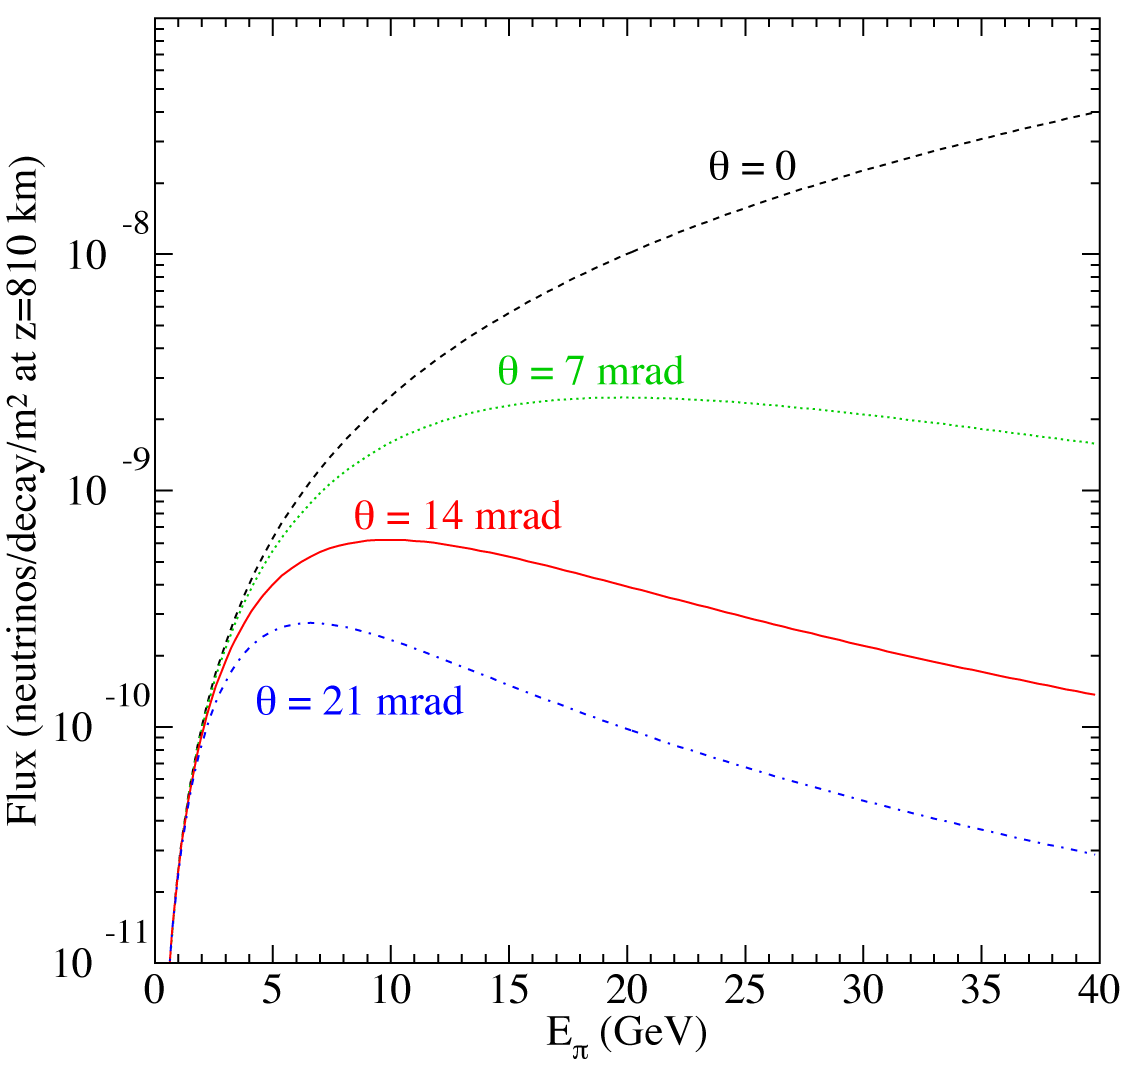
\includegraphics[width=\textwidth]{../../img/baird/beam/020-flux.png}
  \caption{Neutrino flux vs. pion energy. }
  \label{fig:NuPiFluxa}
  \end{subfigure}
  \hfill
  \begin{subfigure}[b]{0.45\textwidth}
  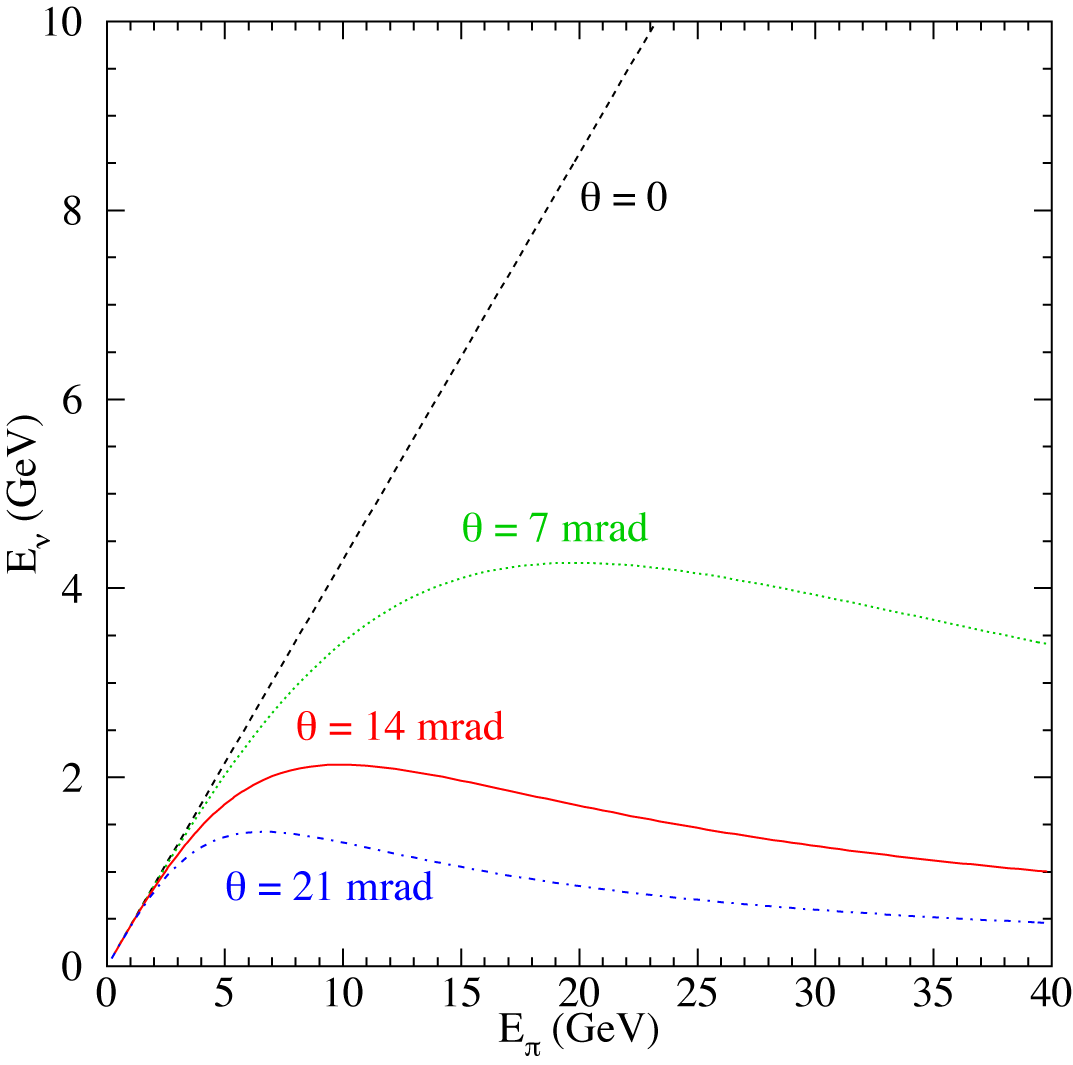
\includegraphics[width=\textwidth]{../../img/baird/beam/030-epi2enu.png}
  \caption{Neutrino energy vs. pion energy.}
  \label{fig:NuPiFluxb}
  \end{subfigure}
  \caption{The above distributions are as viewed from a site located
    800km from the NuMI target and off-axis by an angle $\theta$.}
  \label{fig:NuPiFlux}
\end{figure}



\begin{figure}
  \centering
  \begin{subfigure}[b]{0.45\textwidth}
    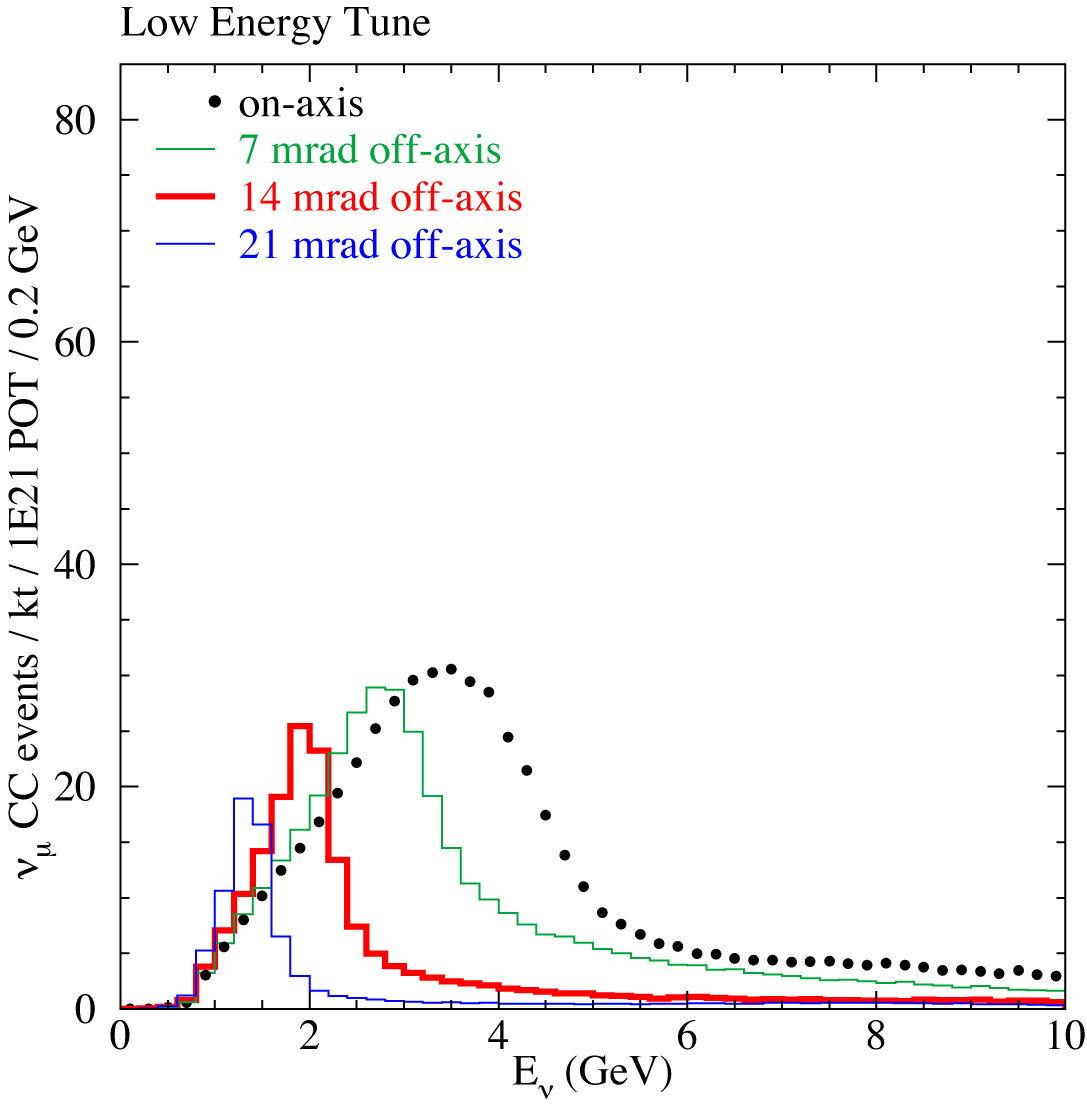
\includegraphics[width=\textwidth]{../../img/baird/beam/040-le-spectra.png}
    \caption{Low Energy Tune neutrino energy.  }
    \label{fig:NuESpectra_MEAndLE_a}
  \end{subfigure}
  \hfill
  \begin{subfigure}[b]{0.45\textwidth}
    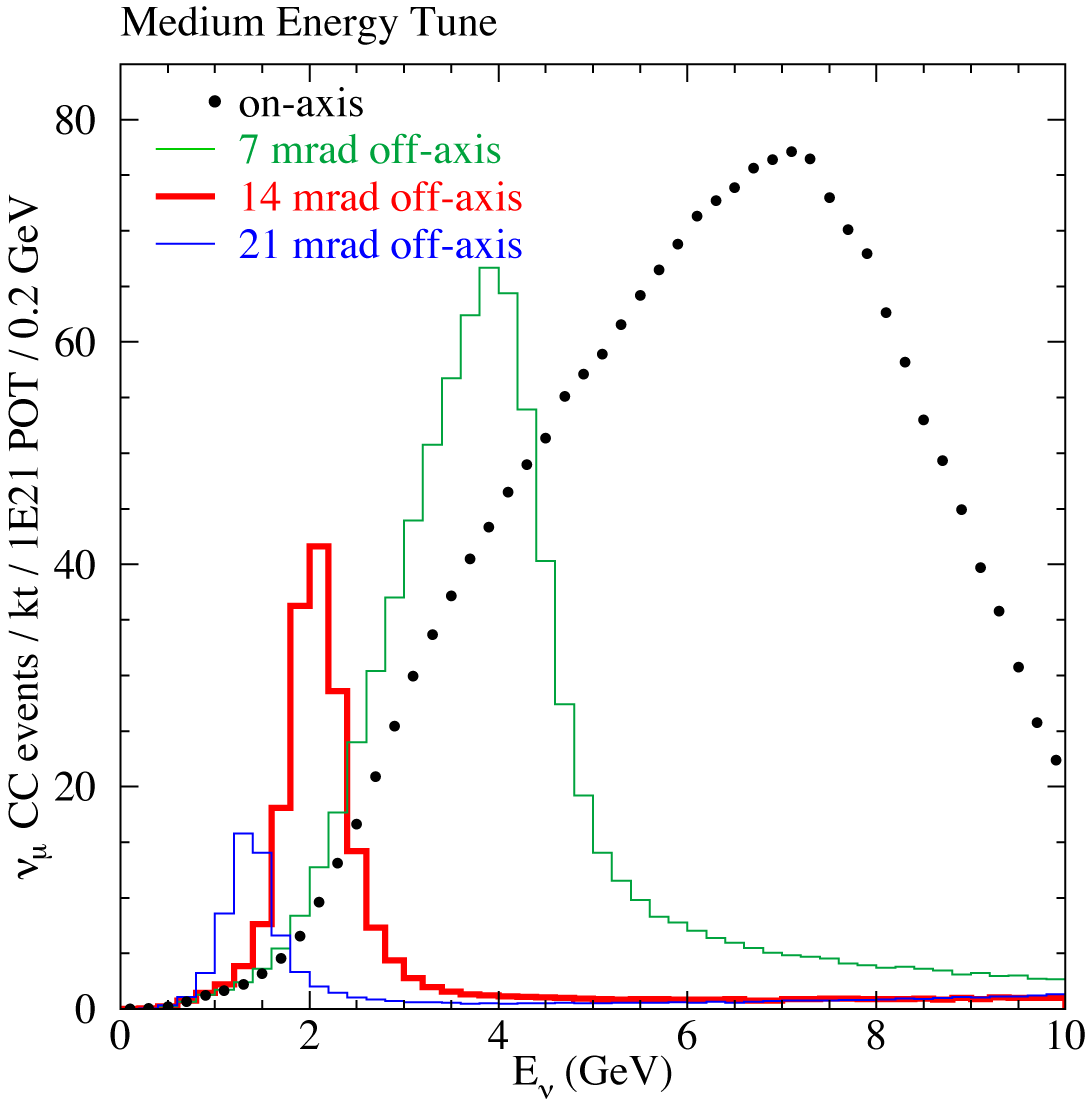
\includegraphics[width=\textwidth]{../../img/baird/beam/050-me-spectra.png}
    \caption{Medium Energy Tune neutrino energy.}
    \label{fig:NuESpectra_MEAndLE_b}
  \end{subfigure}
  \caption{Charged current $\nu_{\mu}$ event rates vs. neutrino
    energy in the absence of oscillations. The distributions are found
  for a detector which is 800~km from the NuMI target and for various
  off-axis angles.}
  \label{fig:NuESpectra_MEAndLE}
\end{figure}


\begin{figure}
  \centering
  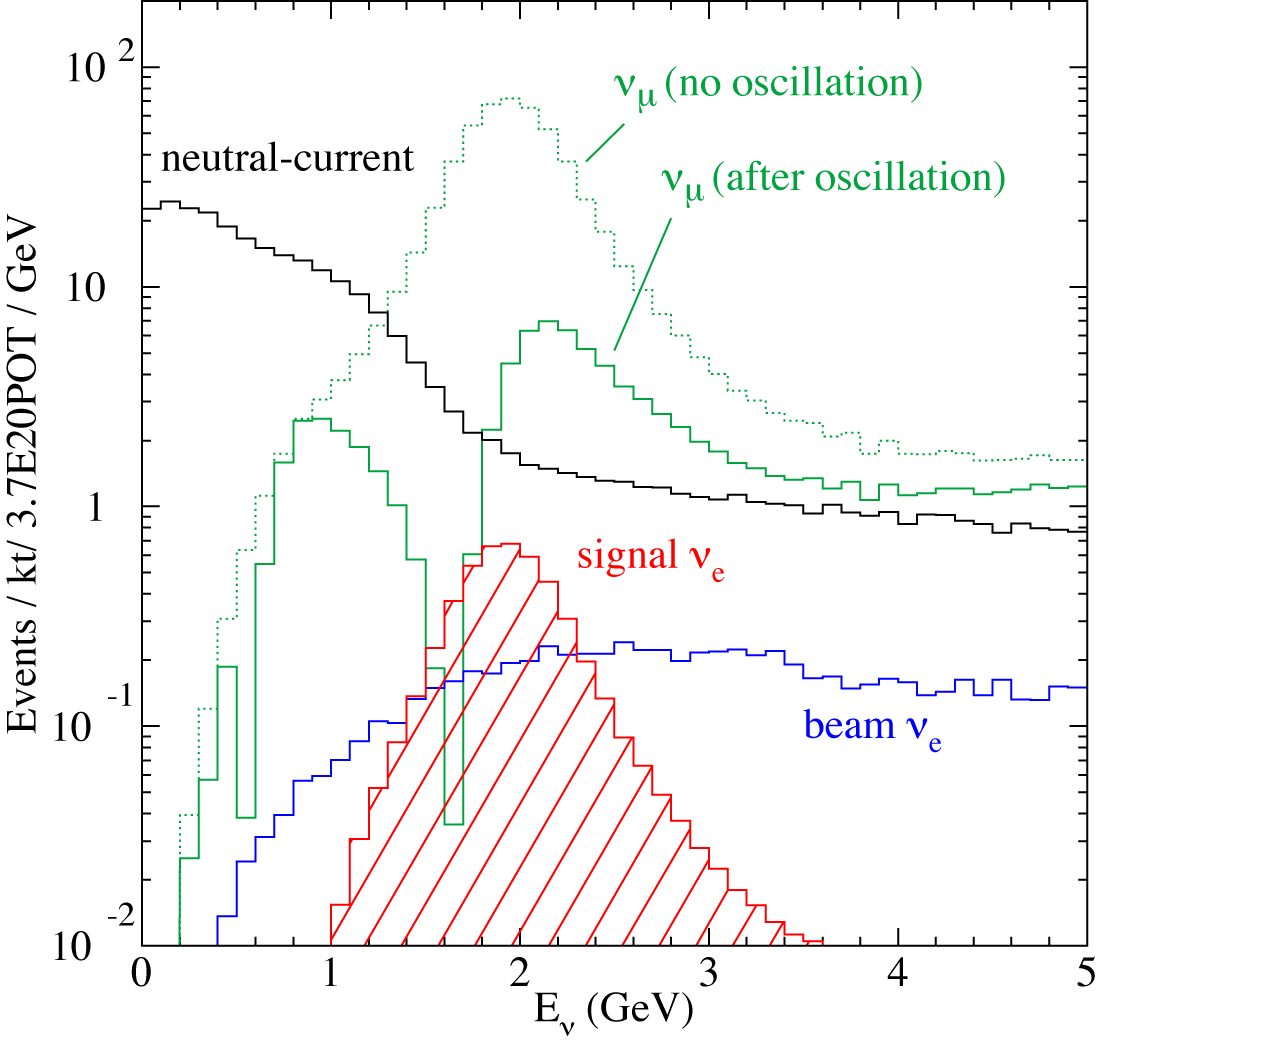
\includegraphics[width=0.5\textwidth]{../../img/beam/060-sig-and-bg-rates-thumb.png}
  \caption{Simulated visible energy distributions for $\nu_{\mu}$ CC
    events with and without oscillations, $\nu_e$ oscillation signal events,
    intrinsic beam $\nu_e$ events and neutral current events. The
    simulation assumes an off-axis position of 12~km at 810~km, $\Delta m^2 = 2.5 \times 10^{-3}
    \textrm{eV}^2$, $\sin^2(2\theta_{23}) = 1.0$ and
  $\sin^2(2\theta_{13}) = 0.1$.}
  \label{fig:NuMIBeamComp}
\end{figure}


\section{The NOvA Detectors}

The NOvA experiment uses a near and far detector to measure neutrino
oscillations. The near detector is used to measure the un-oscillated
neutrino energy spectrum and the electron neutrino component of the
beam. The un-oscillated neutrino energy spectrum measured by the near
detector is extrapolated to the far detector (\textcolor{red}{need to
  discuss further in a future chapter}). The far detectors purpose is
to measure the energy spectrum of the beam neutrinos for comparison
with the extrapolated near detector energy spectrum.

The NOvA experiment aims to perform both $\nu{\mu}$ disappearance and
$nu_e$ appearance measurements. The
detectors are designed to distinguish electron and muon neutrino
charged current events from backgrounds. 

%include all information common among both detectors.
The near and far NOvA detectors are almost functionally
identical. Besides
the different masses there are a few physical
differences. The near detector has a so called ``muon catcher'', has a
higher rate of readout and uses slightly different APDs. The
construction common among both detectors will be discussed in the
following section. The details specific to the far and near detectors
will be discussed in Subsections~\ref{sec:fardet} and
\ref{sec:neardet} respectively.

\subsection{The Basic NOvA Detector Element} \label{sec:cell}

The basic unit of both NOvA detectors is a rectangular rigid PVC cell
which contains liquid scintillator and a wavelength-shifting (WLS)
fibre. An illustration of the cell is shown in
Figure~\ref{fig:cell}. The WLS fibre, which is twice the length of the
cell, is looped at the bottom of the cell such that the captured light
travels in two directions to the instrument top end of the cell. At
the top end of the cell each end of the looped fibre is directed onto
one pixel of an Avalanche Photo Diode (APD) array. The APD converts
the light from the fibre to a digital signal.

The NOvA cells are made from highly reflective titanium dioxide loaded
rigid PVC. The cells have 2 and 4.5~mm thick walls, an interior depth
of 5.9~cm along the beam direction, an interior width of 3.8~cm
transverse to the beam direction and an interior length of 15.5~m.


\subsection{Liquid Scintillator}

Approximately 70\% of the NOvA detector mass is composed of the liquid
scintillator within the cells. The composition of the liquid
scintillator is shown in Figure~\ref{fig:scintComp}. The scintillator
is composed mainly of mineral oil along with 4.1\% pseudocumene as the
scintillant. The scintillant emits scintillation light with a spectrum
peaked between 360 - 390~nm. Wavelength shifting chemical
additives PPE and bis\_MSB are added to shift the initial light
spectrum to 400 - 450~nm to match the absorption spectra of the WLS
fibre. 

\begin{figure}
  \centering
  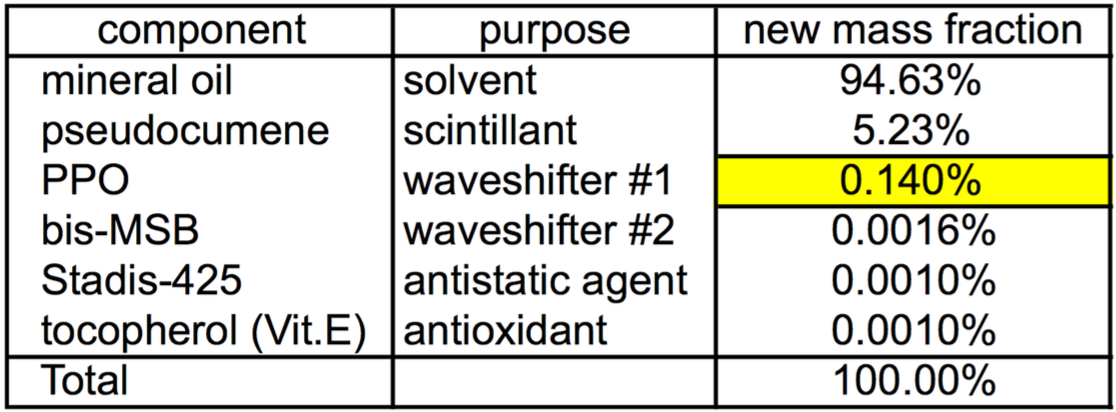
\includegraphics[width=0.8\textwidth]{../../img/det/gen/ScintCompTable.png}
  \caption{Liquid scintillator composition. Table taken from \cite{scintillatorComp}. }
  \label{fig:scintComp}
\end{figure}


\subsection{Wavelength Shifting Fibre}
The WLS fibre has a diameter of 0.7~mm and a core of polystyrene mixed
with 300~ppm R27 dye as the wave shifter. The fibre has two coatings
of materials with a lower refractive index than the core which
facilitates total internal reflection within the fibre. The fibre is
first coated with a thin acrylic layer of PMMA and second with
fluor-acrylic. These coatings make up about 3\% of the fibre
diameter. 

The 400 - 450~nm light emitted by the scintillator is absorbed by the
fibre and wavelength shifted to green light (490 - 550~nm). 
As light travels down the fibre it is attenuated, by a factor of about
10 in the FD, with red light (520 - 550~nm) preferentially
surviving. 


\subsection{Avalanche Photo Diode}

The light exiting the fibre ends is detected by an Avalanche
Photodiode (APD), see Figure~\ref{fig:apd}. An APD contains an array
of 32 pixels, each pixel is interfaced with both ends of a single WLS
fibre. The NOvA APD has an 85\% quantum efficiency for the red light (520 -
550~nm) exiting the fibre ends. 
The thermal noise generated by each APD is reduced by thermo-electric
coolers which cool the APDs to -15$^o$C. The excess heat is removed by
a water cooling system.



\begin{figure}
  \centering
  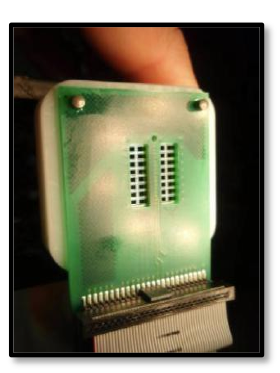
\includegraphics[width=0.4\textwidth]{../../img/det/gen/APD.png}
  \caption{The NOvA APD containing an array of 32 pixels.}
  \label{fig:apd}
\end{figure}


\subsection{Front End Board}

A front end board (FEB) is connected to each APD. The
signals from each APD are continously read out by the FEBs.


\subsection{Detector Assembly} \label{sec:detAssembly}

%build the detector starting with the cell:
The NOvA detectors are constructed from the cells described
in Section~\ref{sec:cell}. 16 cells are extruded together in one unit
to form an extrusion as shown in Figure~\ref{fig:extrusion}. 

Two extrusions are placed side by side to form an extrusion module
consisting of 32 cells as shown in Figure~\ref{fig:module}. The
module ends are capped by the end plate so that the modules can
contain the liquid scintillator. The other end is capped by a manifold
cover which contains the liquid scintillator in the horizontal cells
and directs the 32 fibre end pairs to the 32 APD pixels in the NOvA
APD. 

Flat planes of cells are constructed from multiple modules glued
together side by side. 
The planes layered with alternating orthogonal
orientations, such that the orientation of the cells making up the
plain alternate between horizontal and vertical from plane to plane (see
Figure~\ref{fig:stackedPlanes}). The orthogonal
orientation of the planes allows for three dimensional reconstruction
of tracks passing through multiple planes. Planes are glued together
in the orthogonal arrangement described above to form one solid
detector piece called a block, consisting of 32 or 24 planes in the
far detector or near detector respectively.

%image of cell
\begin{figure}
  \centering
  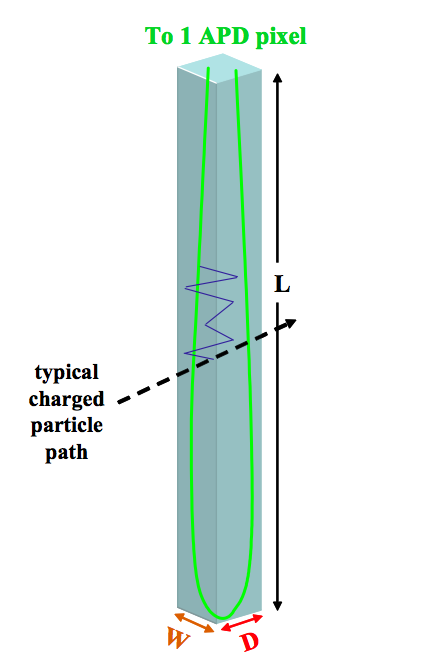
\includegraphics[width=0.5\textwidth]{../../img/det/gen/nova_cell.png}
  \caption{A NOvA cell consisting of an extruded
    PVC tube filled with liquid scintillator and a looped WLS fibre.}
  \label{fig:cell}
\end{figure}


 %extrusion
\begin{figure}
  \centering
  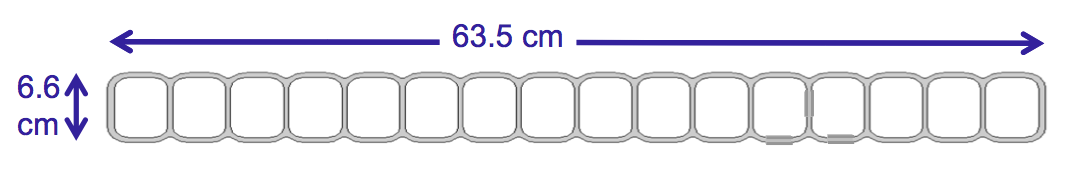
\includegraphics[width=0.5\textwidth]{../../img/det/gen/extru_cross_section.png}
  \caption{A side on view of an extrusion constructed from16 cells.}
  \label{fig:extrusion}
\end{figure}

 %module
\begin{figure}
  \centering
  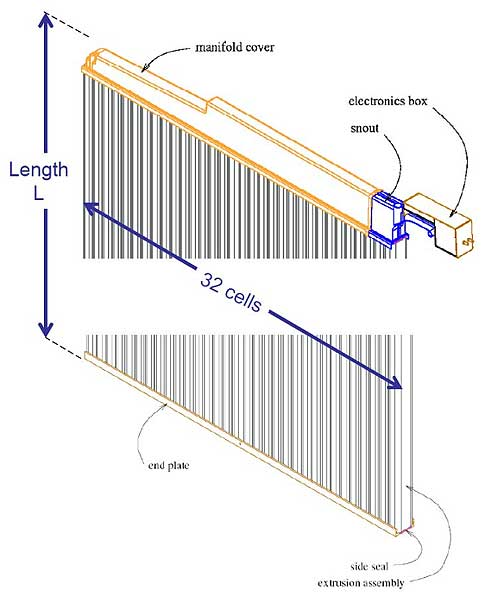
\includegraphics[width=0.5\textwidth]{../../img/det/gen/extrusionModule.jpg}
  \caption{A side on view of an extrusion module constructed from two
    extrusions of 16 cells. }
  \label{fig:module}
\end{figure}

%orthogonally stacked planes
\begin{figure}
  \centering
  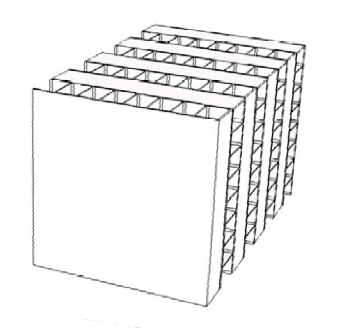
\includegraphics[width=0.5\textwidth]{../../img/det/gen/planes.png}
  \caption{Cut out of a NOvA detector showing the alternating
    orientation of the stacked planes.}
  \label{fig:stackedPlanes}
\end{figure}


\section{Data Acquisition System}

NOvA's readout and data acquisition system (DAQ) are designed to
concentrate data from all the channels into one stream to be analysed
and stored.
Data is stored in an intermediate location while online trigger
processors analyse whether to record or reject the data.



% The data acquisition system (DAQ) starts with the from end boards
% (FEBs) that attach to each APD. 



%Explain digitisation via single and multi point readout.


\subsection{The Far Detector}\label{sec:fardet}

The 14~kt far detector is located 810~km from the NuMI target,
approximately 10~m below the surface and at an elevation of 372~m
above sea-level. The neutrino beam enters the
detector travelling at an angle of 3$^o$ upwards. The detector is
constructed, as described in Section~\ref{sec:detAssembly}, from
344,064 15.5~m long cells which form 896 planes normal to the beam
direction. The detector mass is approximately 65\% liquid scintillator
and 35\% PVC.

As described above, the far detector is built on the surface above sea
level which means that cosmic rays will be a major source of
background events. The background due to cosmic rays is mitigated
using selection cuts and a shielding overburden above the detector.
For the $\nu_{\mu}$ disappearance analysis the background is primarily
due cosmic ray muons which are removed using cuts. For the $\nu_e$
appearance analysis the background is primariy cosmic ray photons
whose interactions within the detector can be mistaken for an electron
shower. 

During a six year run the FD without overburden shielding will see
approximately 1600 background events due to cosmic ray photons. In
order to reduce this background source to less than one event requires
approximately 9 radiation lengths of material above the detector
surface. Additional radiation lengths are desirable to contain any
showers caused by interactions within the overburden. With this in
mind the far detector building was constructed with a 122~cm thick
concrete enclosure which supports a 15~cm thick overburden of
barite. Together, the concrete enclosure and barite overburden provide
12 radiation lengths of shielding.



\subsection{The Near Detector}\label{sec:neardet}

The NOvA near detector is located on site at Fermilab next to the
MINOS Hall as shown in Figure~\ref{fig:cavern}. The detector is 105~m
underground and 1.015~km from the NuMI target. The detector therefore
sees a higher flux of NuMI neutrino events and a lower flux of cosmic
rays than the far detector.
The neutrino beam enters the detector travelling downwards at an angle
of 3$^o$ downwards. 
A diagram of the near detector is shown in Figure~\ref{fig:neardet}.
The detector is constructed in a similar fashion to the far detector
from 20,192 cells arranged in 214 planes, each plane is comprised of 3
modules (except in the muon catcher). The detector has a width and
height of 4.2~m and a length of 15.8~m. The near detector is
functionally equivalent to the far detector with the exception of two
distinguishing features.

First, a muon catcher is employed at the downstream end of the near
detector. 
The muon catcher is constructed from layers of steel planes and
planes of liquid scintillator cells. The steel planes are 10~cm
thick and are seperated by pairs of horizontal and vertically aligned
planes of liquid scintillator cells. The vertical planes consist of
three modules while the horizontal planes are made from just two
modules. Therefore the sets of steel and scintillator planes are
three modules wide (the same as the rest of the detector) but only
two modules high. Ten of these steel and
liquid scintillator plane sets are stacked to form the muon
catcher. The downstream end of the muon catcher has an additional 3
liquid scintillator planes. The muon catcher is added to the
downstream end of the near detector in order to help range out muons
from few GeV charged current $\nu_{\mu}$ interactions.

Second, the near detector electronics are setup to sample each channel
four times more frequently (every 125~ns) than in the far 
detector to help handle the data pileup. 
The near detector sees approximately 5-10 neutrino interactions per
beam spill (10 $\mu s$ window) while the far detector sees
approximately 60-70 cosmic rays per 550 $\mu s$ window spread out over
approximately 17 times more channels. The faster sampling rate
improves the timing resolution of hits in the detector. With better
timing resolution pileup events are more easily distinguished from one
another. 




 %cavern diagram
\begin{figure}
  \centering
  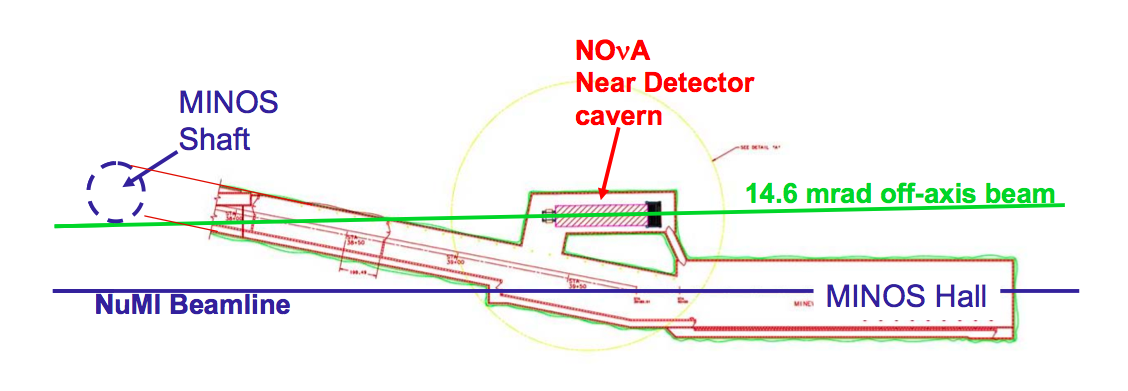
\includegraphics[width=0.8\textwidth]{../../img/baird/det/neardet_cavern_diagram.png}
  \caption{Bird's-eye view of NuMI Beamline, NOvA near detector cavern
    and the MINOS Hall. }
  \label{fig:cavern}
\end{figure}

 %near detector 
\begin{figure}
  \centering
  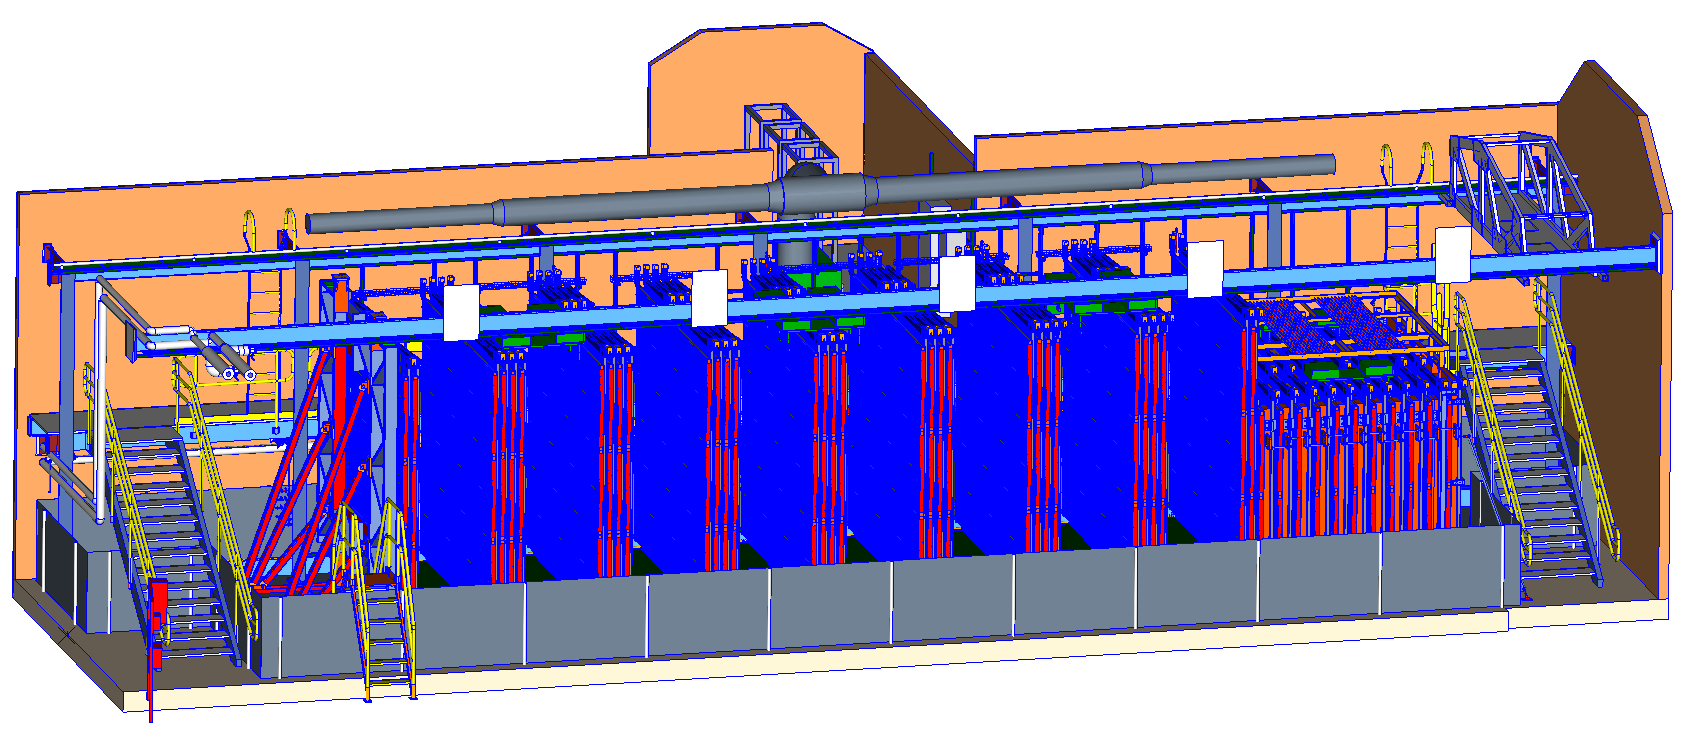
\includegraphics[width=0.8\textwidth]{../../img/baird/det/ND_01.png}
  \caption{Technical drawing of the near detector and surrounding
    cavern. The NuMI beam enters from the left and the shorter muon
    catcher is shown on the right hand side of the detector. Note that
    only some of the planes have been drawn to aid visualisation.}
  \label{fig:neardet}
\end{figure}







